\section{\Zoo[]logy}

\begin{frame}{\Zoo[]logy: what is it?}
\centering
\vspace{5mm}

\begin{tikzpicture}
    \draw [thick, teal] (0,0) rectangle ++(11,6.8) ;
    \draw (3.5,-0.3) node [teal] {\Coq} ;
    
    \draw [thick, orange] (0.2,0.2) rectangle ++(10.6, 6.4) ;
    \draw (5.5, 0) node [orange] {\Iris} ;
    
    \draw [thick, magenta] (0.4,0.4) rectangle ++(10.2, 6) ;
    \draw (7.5, 0.6) node [magenta] {\Zoo} ;
    
    \only<1>{
        \draw (5.5, 3.5) node [magenta] {\vbox{
            \begin{tabular}{l}
                \HeapLang (modified) \\
                + ADTs \\
                + DLS \\
                + exceptions \\
                + algebraic effects \\
                + relaxed memory \\\\
                (planned before \Osiris, \\
                in case you were wondering)
            \end{tabular}
        }} ;
    }
    
    \only<2->{
        \draw [thick, blue] (0.8,1.8) rectangle ++(1.5,1) node [midway] {\Std} ;
    }
    
    \only<3->{
        \draw [thick, cyan] (0.8,3.8) rectangle ++(1.5,1) node [midway] {\Pstore} ;
    }
    
    \only<5->{
        \draw [thick, olive] (3,1.2) rectangle ++(5,4.2) node [midway] {\vbox{
            \texttt{Mpmc\_stack} \\
            \texttt{Mpmc\_queue} \\
            \texttt{Mpsc\_queue} \\
            \texttt{Ws\_deque} \\
            \texttt{Skiplist} \\
            \texttt{Htbl} \\
            \dots
        }} ;
        \draw (5.5,5.8) node [olive] {\Saturn} ;
    }
    
    \only<7->{
        \draw [thick, brown] (8.7,3.8) rectangle ++(1.5,1) node [midway] {\Parabs} ;
    }
    
    \only<8->{
        \draw [thick, violet] (8.7,1.8) rectangle ++(1.5,1) node [midway] {\Kcas} ;
    }
\end{tikzpicture}

\begin{overbox}<4>
    \begin{figure}
        \begin{subfigure}{0.4\textwidth}
            
\includegraphics[scale=0.4]{images/basile_clement.jpg}
            \caption*{\footnotesize Basile \\ Clément}
        \end{subfigure}
        \begin{subfigure}{0.3\textwidth}
            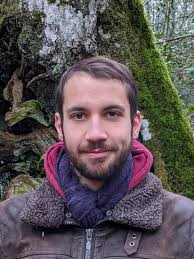
\includegraphics[scale=0.3]{images/alexandre_moine.jpg}
            \caption*{\footnotesize Alexandre \\ Moine}
        \end{subfigure}
        \begin{subfigure}{0.25\textwidth}
            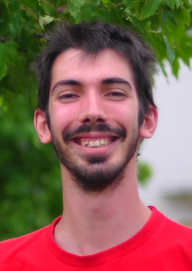
\includegraphics[scale=1.2]{images/gabriel_scherer.jpg}
            \caption*{\footnotesize Gabriel \\ Scherer}
        \end{subfigure}
        \caption*{The \Pstore team!}
    \end{figure}
\end{overbox}

\begin{overbox}<6>
    \begin{figure}
        \begin{subfigure}{0.4\textwidth}
            
\includegraphics[scale=0.2]{images/vesa_karvonen.jpg}
            \caption*{\footnotesize Vesa Karvonen}
        \end{subfigure}
        \begin{subfigure}{0.4\textwidth}
            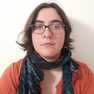
\includegraphics[scale=1]{images/carine_morel.jpg}
            \caption*{\footnotesize Carine Morel}
        \end{subfigure}
        \caption*{The \Saturn team!}
    \end{figure}
\end{overbox}

\begin{overbox}<9>
    \begin{figure}
        \begin{subfigure}{0.4\textwidth}
            
\includegraphics[scale=0.2]{images/vesa_karvonen.jpg}
            \caption*{\footnotesize Vesa Karvonen}
        \end{subfigure}
        \caption*{The main author of \Kcas!}
    \end{figure}
\end{overbox}
\end{frame}

\begin{frame}{\Zoo[]logy: why is it fun?}
Lockfree algorithms typically exhibit complex behaviors:
\begin{itemize}
    \item physical state $\neq$ logical state,
    \item external linearization points,
    \item future-dependent linearization points.
\end{itemize}
\vfill
\Iris is a good match for verifying them thanks to advanced mechanisms:
\begin{itemize}
    \item invariants to enforce protocols,
    \item atomic updates to materialize linearization points,
    \item prophecy variables to reason on the future.
\end{itemize}
\end{frame}